\documentclass[oupdraft]{bio}
% \usepackage[colorlinks=true, urlcolor=citecolor, linkcolor=citecolor, citecolor=citecolor]{hyperref}
\usepackage{url}
\usepackage{longtable}
\usepackage{multirow}
\usepackage[T1]{fontenc}
\usepackage[utf8]{inputenc}
\usepackage[table]{xcolor}


\newcommand\independent{\protect\mathpalette{\protect\independenT}{\perp}}
\def\independenT#1#2{\mathrel{\rlap{$#1#2$}\mkern2mu{#1#2}}}

\usepackage{tikz}
\usetikzlibrary{shapes}
\usepgflibrary{plotmarks}
\usetikzlibrary{plotmarks}


\newcommand{\mysquare}[1]{\tikz{\node[draw=#1,fill=#1,rectangle,minimum
width=0.18cm,minimum height=0.18cm,inner sep=0pt] at (0,0) {};}}

\newcommand{\mycircle}[1]{\tikz{\node[draw=#1,fill=#1,circle,minimum
width=0.2cm,minimum height=0.2cm,inner sep=0pt] at (0,0) {};}}

\newcommand{\mystar}[1]{\tikz{\node[draw=#1,fill=#1,star,minimum
width=0.2cm,minimum height=0.2cm,inner sep=0pt] at (0,0) {};}}

\newcommand{\mytriangle}[1]{\tikz{\node[draw=#1,fill=#1,isosceles
triangle,isosceles triangle stretches,shape border rotate=90,minimum
width=0.2cm,minimum height=0.2cm,inner sep=0pt] at (0,0) {};}}

% Add history information for the article if required
\history{Received August 1, 2010;
revised October 1, 2010;
accepted for publication November 1, 2010}

\begin{document}

% Title of paper
\title{It's all about balance: propensity score matching in the context of complex survey data}

% List of authors, with corresponding author marked by asterisk
\author{DAVID LENIS$^\ast$\\
% Author addresses
\textit{Department of Biostatistics, Johns Hopkins Bloomberg School of Public Health, Baltimore, MD 21205, USA}\\
% E-mail address for correspondence
{dlenis@jhsph.edu}\\
TRANG Q. NGUYEN\\
\textit{Departments of Mental Health, Johns Hopkins Bloomberg School of Public Health, Baltimore, MD 21205, USA}\\
NIANBO DONG\\
\textit{Department of Educational, School and Counseling Psychology, University of Missouri, Columbia, MO 65211, USA}\\
ELIZABETH A. STUART\\
\textit{Departments of Mental Health, Biostatistics, and Health Policy and Management, Johns Hopkins Bloomberg School of Public Health, Baltimore, MD 21205, USA}}

% Running headers of paper:
\markboth%
% First field is the short list of authors
{D. Lenis and others}
% Second field is the short title of the paper
{Propensity Score Matching with Complex Survey Data}
\maketitle

% Add a footnote for the corresponding author if one has been
% identified in the author list
\footnotetext{To whom correspondence should be addressed.}


\section*{Appendix A: Non-response mechanisms}
Traditionally, missing data mechanisms are grouped in three categories: (1) Missing Completely at Random (MCAR), (2) Missing and Random (MAR) and (3) Missing not at Random (MNAR). Under a MCAR mechanism, the probability that one observation will have missing information, is completely random. In other words, there is no relationship between the propensity of the data to be missing and the values of the variables in the data set. When the non-response follows a MAR mechanism, the propensity of the data to be missing is random, conditional on the set of observed variables. In other words the observed values of the available data, can predict the probability of one observation to have missing information. Finally when the non-response is MNAR, the probability of having missing information depends on unobserved variables. That is, even after accounting for the observed variables available in the data, the propensity of the data to be missing is not random.    

\section*{Appendix B: Non-response and Survey Weights}

The survey weights, $\omega$, are equal to the inverse of the probability of being observed in the sample,
formally:
\begin{equation}
\omega=\frac{1}{p}=\frac{1}{f_{SR|(\mathbf{X},T)}\left(SR=1|\mathbf{X},T\right)}\label{eq:WEIG}
\end{equation}

Notice that this definition allows for a non-response rate different from 0 and different non-response mechanisms. To see this, consider the case where $S$ and  $R$ are independent conditional on $(\mathbf{X},T)$. Then it holds that $f_{SR|(\mathbf{X},T)}\left(SR=1|\mathbf{X},T\right)$ it's equal to $f_{S|(\mathbf{X},T)}\left(S=1|\mathbf{X},T\right)$ times $f_{R|(\mathbf{X},T)}\left(R=1|\mathbf{X},T\right) $, this last term models the non-response mechanism. Notice that if $f_{R|(\mathbf{X},T)}\left(R=1|\mathbf{X},T\right) = 1$ for all $(\mathbf{x},t)$ in $(\mathbf{X},T)$ then the non-response rate is 0. If $f_{R|(\mathbf{X},T)}\left(R=1|\mathbf{X},T\right) = f_{R}\left(R=1\right)$ the non-respond mechanism is MCAR. Finally, the non response could be MAR and NMAR depending on whether the all the elements in $\left(\mathbf{X},T\right)$ are observed. If every element in $\left(\mathbf{X},T\right)$ is available to estimate the probability of non-response, then the non-response mechanism is MAR, otherwise the non-response process is NMAR. In this way, $\omega$ (the final observed sampling weight) is a combination of the survey weights associated with the sampling design itself but also incorporates corrections associated with non-response. 

\section*{Appendix C: Estimating the PATT}
\label{AA}
Here we incorporate the weight transfer to estimate the PATT. The PATT will be estimated as the difference of the weighted mean of the observed outcomes of the treated and their matched comparison units. This estimator of the PATT makes the use of the weights explicit, nevertheless it is important to recall that a outcome model can be defined and the weights can be incorporated in its estimation. Under the assumption that a $k:1$ matching procedure was implemented it holds that for every
treated unit $j$ with $j=1,2,\ldots,n_{T}=\sum_{i=1}^{N}SR_{i}\times T_{i}$
, we have $h(j)=1,2,\ldots k$ comparison units. Thus the $PATT$ can be computed
by 

\begin{eqnarray*}
\widehat{PATT} & = & \frac{\sum_{j=1}^{n_{T}}y_{j}\times\omega_{j}^{t}(\mathbf{x})}{\sum_{j=1}^{n_{T}}\omega_{j}^{t}(\mathbf{x})}-\frac{\sum_{j=1}^{n_{T}}\sum_{h(j)=1}^{k}y_{h(j)}\times\omega_{j}^{t}(\mathbf{x})}{\sum_{j=1}^{n_{T}}\sum_{h(j)=1}^{k}\omega_{j}^{t}(\mathbf{x})}\\
 & = & \frac{\sum_{j=1}^{n_{T}}y_{j}\times\omega_{j}^{t}(\mathbf{x})}{\sum_{j=1}^{n_{T}}\omega_{j}^{t}(\mathbf{x})}-\frac{\sum_{j=1}^{n_{T}}\sum_{h(j)=1}^{k}y_{h(j)}\times\omega_{j}^{t}(\mathbf{x})}{\sum_{h(1)=1}^{k}\omega_{1}^{t}(\mathbf{x})+\sum_{h(2)=1}^{k}\omega_{2}^{t}(\mathbf{x})+...+\sum_{h(n_{T})=1}^{k}\omega_{n_{T}}^{t}(\mathbf{x})}\\
 & = & \frac{\sum_{j=1}^{n_{T}}y_{j}\times\omega_{j}^{t}(\mathbf{x})}{\sum_{j=1}^{n_{T}}\omega_{j}^{t}(\mathbf{x})}-\frac{\sum_{j=1}^{n_{T}}\sum_{h(j)=1}^{k}y_{h(j)}\times\omega_{j}^{t}(\mathbf{x})}{k\omega_{1}^{t}(\mathbf{x})+k\omega_{2}^{t}(\mathbf{x})+...+k\omega_{n_{T}}^{t}(\mathbf{x})}\\
& = & \frac{\sum_{j=1}^{n_{T}}y_{j}\times\omega_{j}^{t}(\mathbf{x})}{\sum_{j=1}^{n_{T}}\omega_{j}^{t}(\mathbf{x})}-\frac{\sum_{j=1}^{n_{T}}\sum_{h(j)=1}^{k}y_{h(j)}\times\omega_{j}^{t}(\mathbf{x})}{k\sum_{j=1}^{n_{T}}\omega_{j}^{t}(\mathbf{x})}\\
 & = & \sum_{j=1}^{n_{T}}\left[y_{j}\times\frac{\omega_{j}^{t}(\mathbf{x})}{\sum_{j=1}^{n_{T}}\omega_{j}^{t}(\mathbf{x})}\right]-\sum_{j=1}^{n_{T}}\sum_{h(j)=1}^{k}\left[y_{h(j)}\times\frac{\omega_{j}^{t}(\mathbf{x})}{k\sum_{j=1}^{n_{T}}\omega_{j}^{t}(\mathbf{x})}\right]\\
 & = & \sum_{j=1}^{n_{T}}y_{j}\times W_{j}^{t}-\sum_{j=1}^{n_{T}}\sum_{h(j)=1}^{k}y_{h(j)}\times W_{j}^{c}
\end{eqnarray*}


Defining

\begin{eqnarray*}
W_{j}^{t} & = & \frac{\omega_{j}^{t}(\mathbf{x})}{\sum_{j=1}^{n_{T}}\omega_{j}^{t}(\mathbf{x})}\\
W_{j}^{c} & = & \frac{\omega_{j}^{t}(\mathbf{x})}{k\sum_{j=1}^{n_{T}}\omega_{j}^{t}(\mathbf{x})}
\end{eqnarray*}


We can conclude that

\begin{eqnarray*}
W_{j}^{c} & = & \frac{1}{k}W_{j}^{t}
\end{eqnarray*}

Notice that each of the $n_{T}$ treated units receives a weight of $W_{j}^{t}$ and each of the comparison units a weight of $\frac{1}{k}W_{j}^{t}$. Interestingly, when this weight transfer is implemented and then the PATT is estimated, we find that the estimation procedure assigns to each unit of the comparison group a final weight that is proportional to the final weight received by the treated unit to which they have been matched to. Such proportion is defined by the number of comparison units used to matched each treated unit. Notice that a similar result is obtained when considering simple random samples, see \citet{stuart2010matching}. 



\section*{Appendix D: Simulation Study}
As in \citet{austin2016propensity}, we consider the case of a population of size $N=1,000,000$. There are $10$ strata in the population, each stratum has a total of $100,000$ observations. Within each strata there are 20 clusters, each of is composed of $5,000$ units. There are \textbf{six covariates} $X_{l}$ with $l=1,...,6$ and the data generating mechanism for the baseline covariates is such that: (1) the probability density function is normal, (2) the covariates are independent (i.e., correlation between any pair of covariates is set equal to $0$), (3) the standard deviation, across all the covariates, is equal to $1$ and (4) the means vary across strata and cluster. More explicitly, for each strata $\left(j\right)$, the mean of the covariates deviates in $\mu_{lj}$ from $0$, where $\mu_{lj}$ are obtained assuming that $\mu_{lj}\sim N\left(0,\tau^{stratum}\right)$. Within each strata, the mean of each cluster $\left(k\right)$ deviates from the strata specific mean by $\mu_{lk}$, with $\mu_{lk}\sim N\left(0,\tau^{cluster}\right)$.
Thus the distribution of the $l^{th}$ variable, in the $j^{th}$ stratum, among the units of the $k^{th}$ cluster is $X_{l,ijk}\sim N\left(\mu_{lj}+\mu_{lk},\,\,\,1\right)$.
We set $\tau^{stratum}=0.35$ and $\tau^{cluster}=0.25,\,\,0.15,\,\,0.05$. Each value of $\tau^{cluster}$ defines a different scenario. Unless otherwise specified, values of the population coefficients are the ones used by \citet{austin2016propensity} 

The \textbf{treatment assignment} $\left(T_{i}\right)$ model is defined as
a Bernoulli random variable $T_{i}\sim Be\left(p_{i}\right)$ with $logit\left(p_{i}\right)=\alpha_{0}+\sum_{l=1}^{6}\alpha_{l}X_{l,i}$ with $\alpha_{0}=log\left(\frac{0.3290}{0.9671}\right)$, $\alpha_{1}=log(1.10)$,
$\alpha_{2}=log(1.25)$, $\alpha_{3}=log(1.50)$, $\alpha_{4}=log(1.75)$,
$\alpha_{5}=log(2.00)$ and $\alpha_{6}=log(2.50)$. 

The \textbf{potential outcomes} models are defined as 
$Y_{i}\left(0\right)=\beta_{0}+\sum_{l=1}^{6}\beta_{l}X_{1,i}+\epsilon$ with $\epsilon\sim N\text{\ensuremath{\left(0,1\right)}}$ and $\beta_{0}=0$, $\beta_{1}=2.50$, $\beta_{1}=-2.00$, $\beta_{3}=1.75$,
$\beta_{4}=-1.25,$ and $\beta_{6}=1.10$. The potential outcome under
treatment is defined by $Y_{i}\left(1\right)=Y_{i}\left(0\right)+\delta_{0}+\delta_{1}\sum_{l=1}^{3}\beta_{l}X_{l,i}+\sum_{j=1}^{10}\eta_{j}STR_{j,i}$ with $\delta_{0}=1$ and $\delta_{1}=0.2$. The term $\sum_{j=1}^{10}\eta_{j}STR_{j,i}$ is the first departure form the simulation set-up design by \citet{austin2016propensity}. This additional term allows us to control how different  the PATT and the SATT are. The variable $STR_{j,i}$ is a categorical variable that takes the value $1$ if the sample unit $i$ belongs to the $j^{th}$ stratum.  For each of the three scenarios we consider six different values for the vector of parameters $\left(\eta_{1},...,\eta_{10}\right)$ such that $\left(\frac{SATT}{PATT}-1\right)\times100$ takes roughly the values $-50\%, -40\%, -30\%, -20\%, -10\%$ and $0\%$ . 
In addition to a continuous outcome \citet{austin2016propensity} also considered a dichotomous outcome; in our article, we restrict our attention to continuous outcomes.  
We define an indicator variable $R_{m}$ with $m=1,2,3,4$ which takes the value $1$ is the unit responded and $0$ otherwise.  
We consider the following non-response cases: No-missing data (\textbf{NM}), $R_{1i}=1$ for all $i$. Missing at Random (\textbf{MAR}): the non-response rate depends on the six baseline covariates, explicitly we assume that $R_{3i}\sim Be(p_{3i})$ with
$logit\left(p_{3i}\right)=\gamma_{0}+\sum_{l=1}^{6}\gamma_{l}X_{l,i}$ and $\gamma_{0}=-log(0.030)$, $\gamma_{1}=-log(1.10),$ $\gamma_{2}=-log(1.25)$,
$\gamma_{3}=-log(1.50),$ $\gamma_{4}=-log(1.75),$ $\gamma_{5}=-log(2.00),$
$\gamma_{6}=-log(2.50)$. Missing at Random with an additional covariate $X_{7}$ (\textbf{MARX}): the non-response rate depends on the baseline covariates but additionally, depends on a covariate $X_{7}$ that is not observed in the final sample, but affect the response rate. Formally,$R_{3i}\sim Be(p_{3i})$ with $logit\left(p_{3i}\right)=\gamma_{0}+\sum_{l=1}^{7}\gamma_{l}X_{l,i}$ where $\gamma_{7} = -log(2.50)$. This non-response mechanism, aims to model the situation in which the survey weights can are constructed using information that is only available to the survey team (i.e., $X_{7}$), but not available to the final user (e.g., number of contact attempts). The data generating mechanism for the covariate $X_{7}$ is the same as the one for the baseline covariates. The final non-response mechanism consider is Missing at Random where the non-response depends on the baseline covariates and the treatment assignment (\textbf{MART}). Explicitly $R_{4i}\sim Be(p_{4i})$ with $logit\left(p_{3i}\right)=\gamma_{0}+\sum_{l=1}^{6}\gamma_{l}X_{l,i}+\Delta T_{i}$ and $\Delta=-2$.

\section*{Appendix E: Software}
The simulation study and the application were implemented using the software R and the platform RStudio \citep{rstudio2015rstudio}. The following packages were used:  `data.table' \citep{dowle2015datatable}, `ggplot2' \citep{wickham2009ggplot2}, `MatchIt' \citep{ho2011matchit}, `survey' \citep{lumley2015survey}, `sampling' \citep{yves2015} and `xtable' \citep{dahl2016}. 

\section*{Appendix F: Additional plots}
Figures \ref{Diagnostics2} and \ref{Diagnostics3} summarizes our main findings, in terms of the balance achieved by every propensity score matching strategy, for Scenarios 2 and 3 respectively.
Figures \ref{Scenario2} and \ref{Scenario3} summarizes our main findings, related to the performance of each propensity score matching estimator, for Scenarios 2 and 3 respectively.



\begin{figure}[t]
\centering
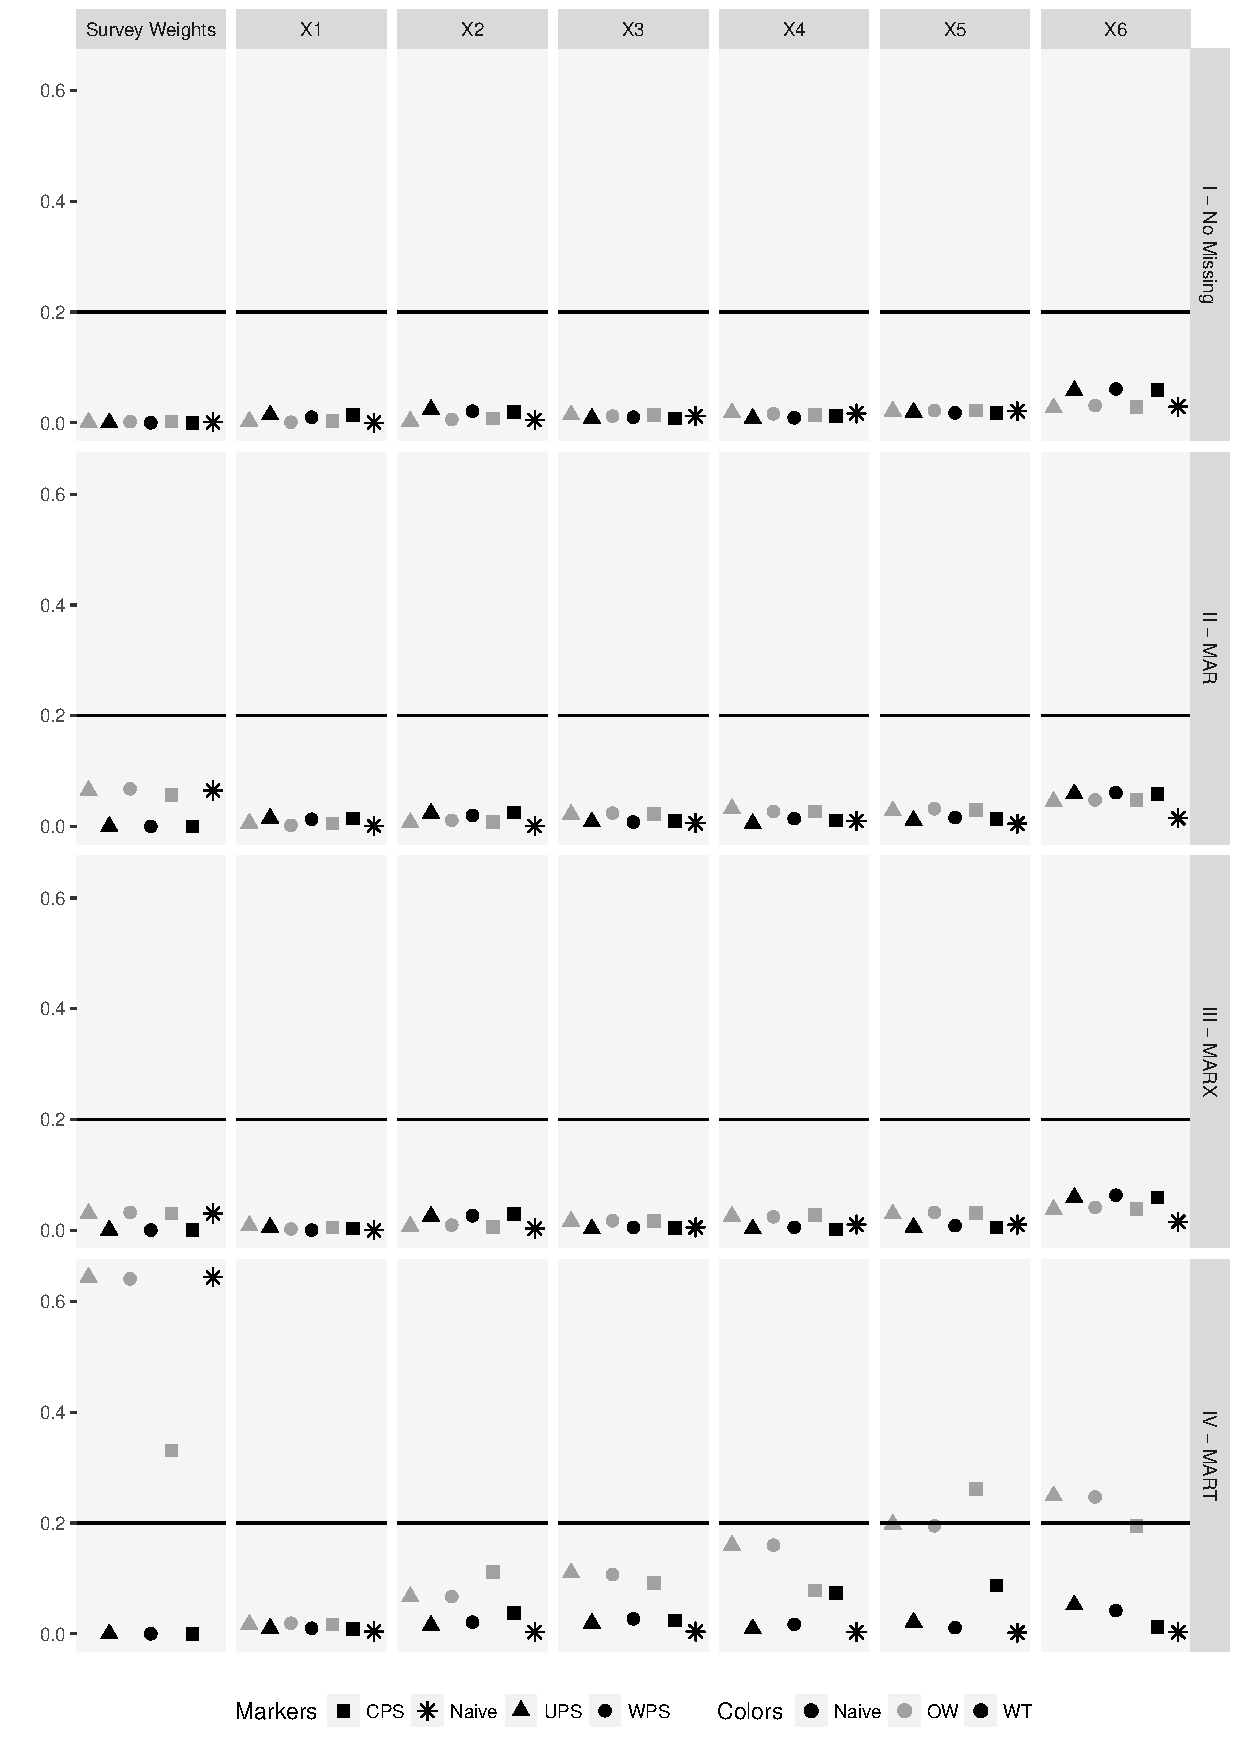
\includegraphics[scale=0.63]{SMD_SC2_v2.pdf}
\caption{{\small{}\textbf{Diagnostics: Scenario 2.} Average SMD, 3ach marker represents how the survey weights were incorporated in estimation of the propensity score model: (\mytriangle{black}) survey weights were not used in the estimation of the propensity score model, but the sample weights are used in the computation of the SMD after matching, (\mycircle{black}) survey weights were incorporated in a weighted estimation of the propensity score model and (\mysquare{black})  survey weights were used as a covariate in the estimation of the propensity score model. Black markers are associated with the weight transfer described in the main manuscript, gray markers show the balance achieved original survey weights are used. We also display the SMD achieved by the Naive estimator using a black asterisk.}}
\label{Diagnostics2} 
\end{figure}

\begin{figure}[t]
\centering
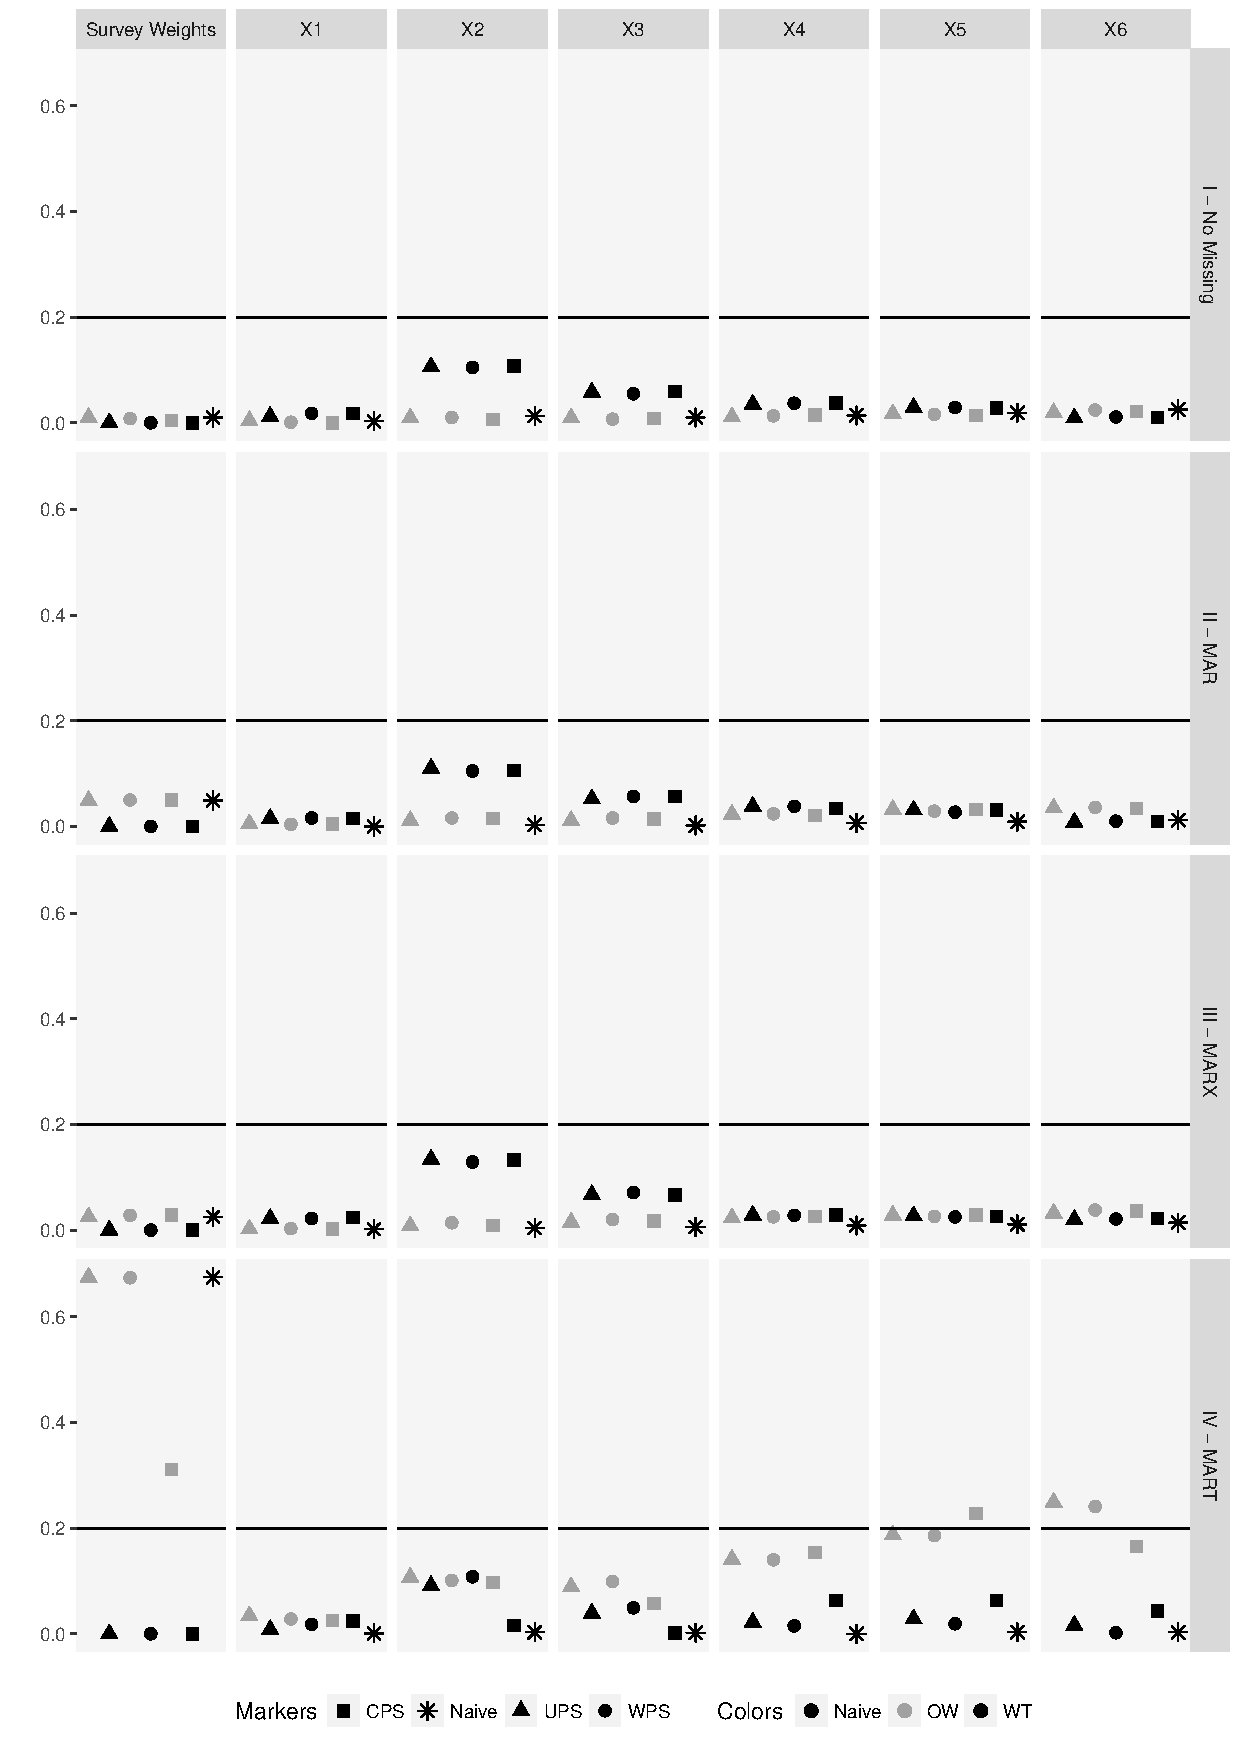
\includegraphics[scale=0.63]{SMD_SC3_v2.pdf}
\caption{{\small{}\textbf{Diagnostics: Scenario 3.} Average SMD, each marker represents how the survey weights were incorporated in estimation of the propensity score model: (\mytriangle{black}) survey weights were not used in the estimation of the propensity score model, but the sample weights are used in the computation of the SMD after matching, (\mycircle{black}) survey weights were incorporated in a weighted estimation of the propensity score model and (\mysquare{black})  survey weights were used as a covariate in the estimation of the propensity score model. Black markers are associated with the weight transfer described in the main manuscript, gray markers show the balance achieved original survey weights are used. We also display the SMD achieved by the Naive estimator using a black asterisk.}}
\label{Diagnostics3} 
\end{figure}


\begin{figure}[t]
\centering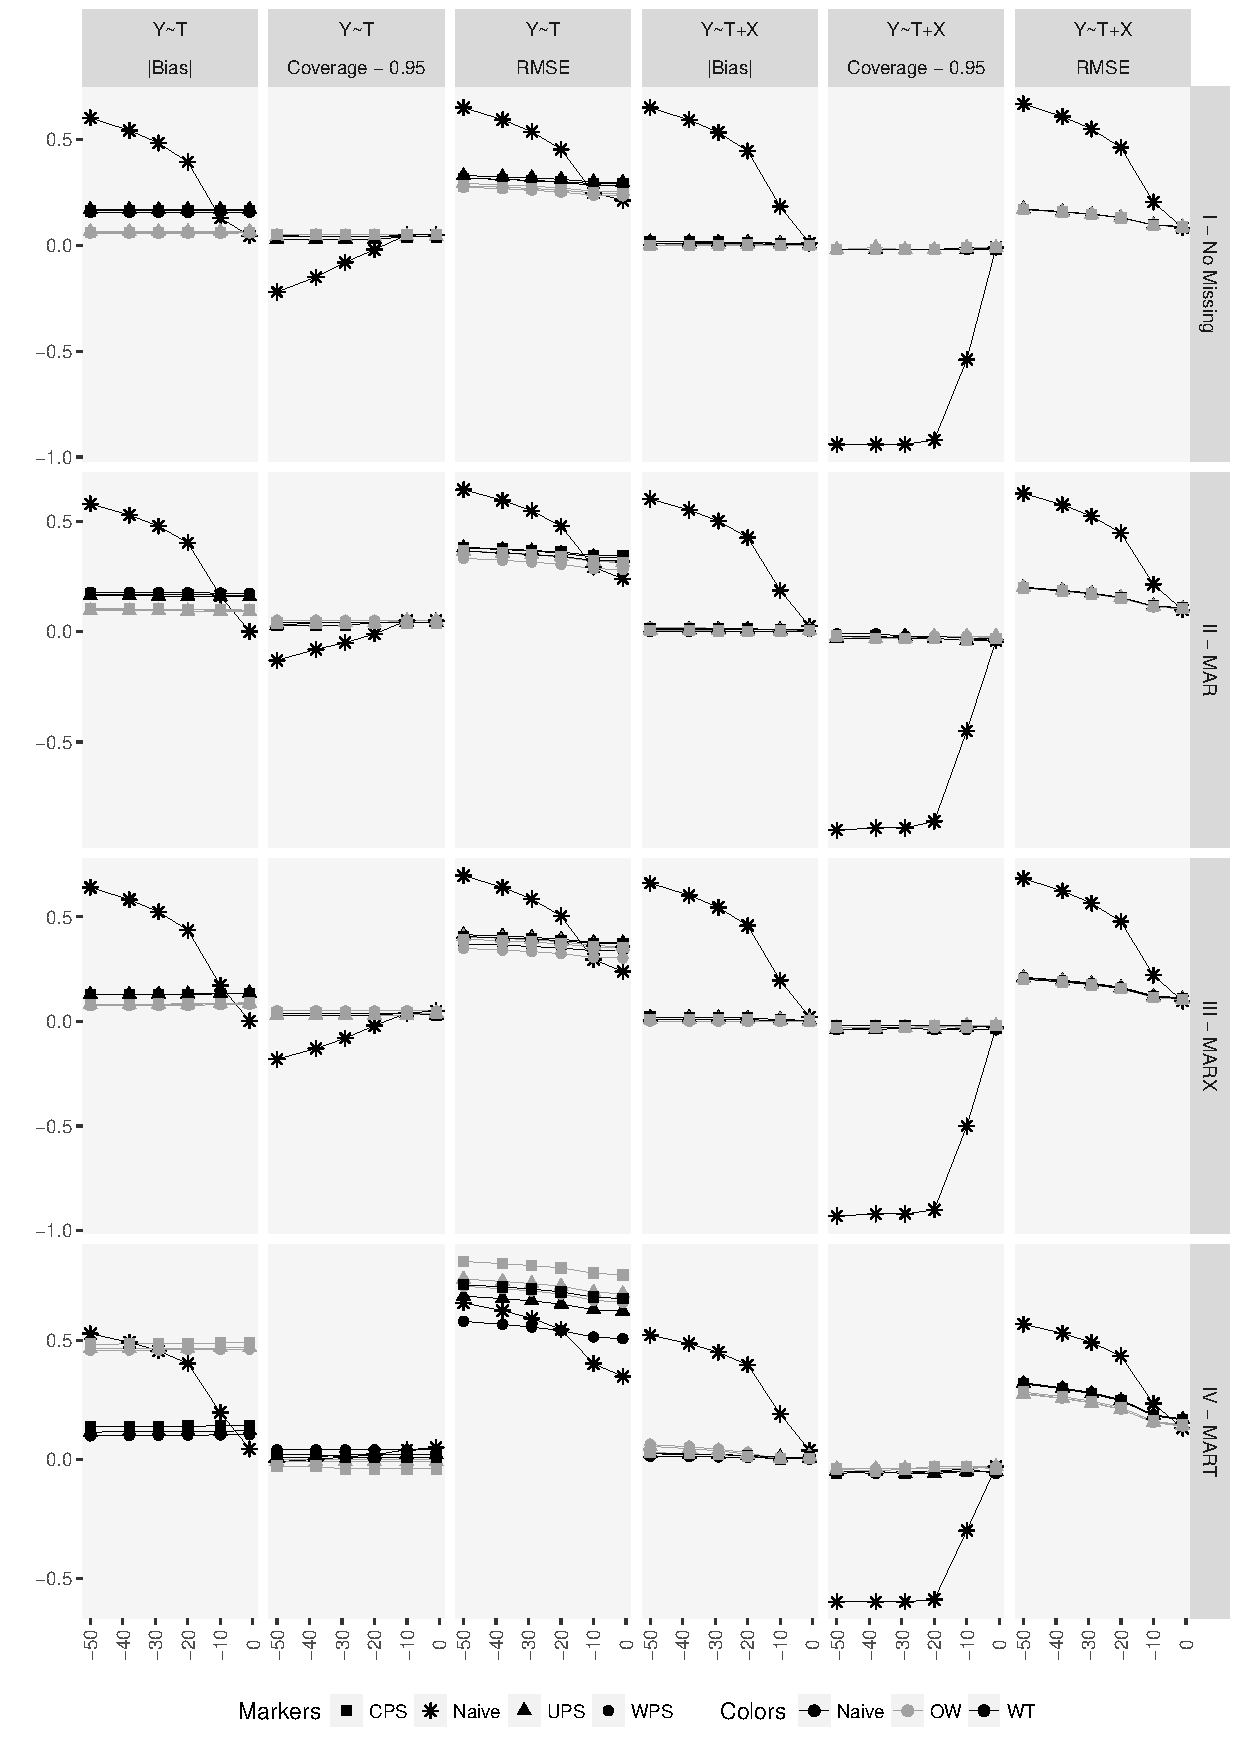
\includegraphics[scale=0.63]{Scenario2_v2.pdf}
\caption{{\small{}\textbf{Results: Scenario 2.} Bias in absolute value, coverage and root mean squared error (RMSE) as functions
of the \% difference between the SATT and PATT (simulation study).Each marker represents how the survey weights were incorporated in estimation of the propensity score model: (\mytriangle{black}) survey weights were not used in the estimation of the propensity score model, but the sample weights are used in the computation of the SMD after matching, (\mycircle{black}) survey weights were incorporated in a weighted estimation of the propensity score model and (\mysquare{black})  survey weights were used as a covariate in the estimation of the propensity score model. Black lines  show the results when the wight transfer is implemented, gray lines show the results when the original survey weights are used. Results for the Naive estimator are displayed using a black asterisk.}}
\label{Scenario2} 
\end{figure}

\begin{figure}[t]
\centering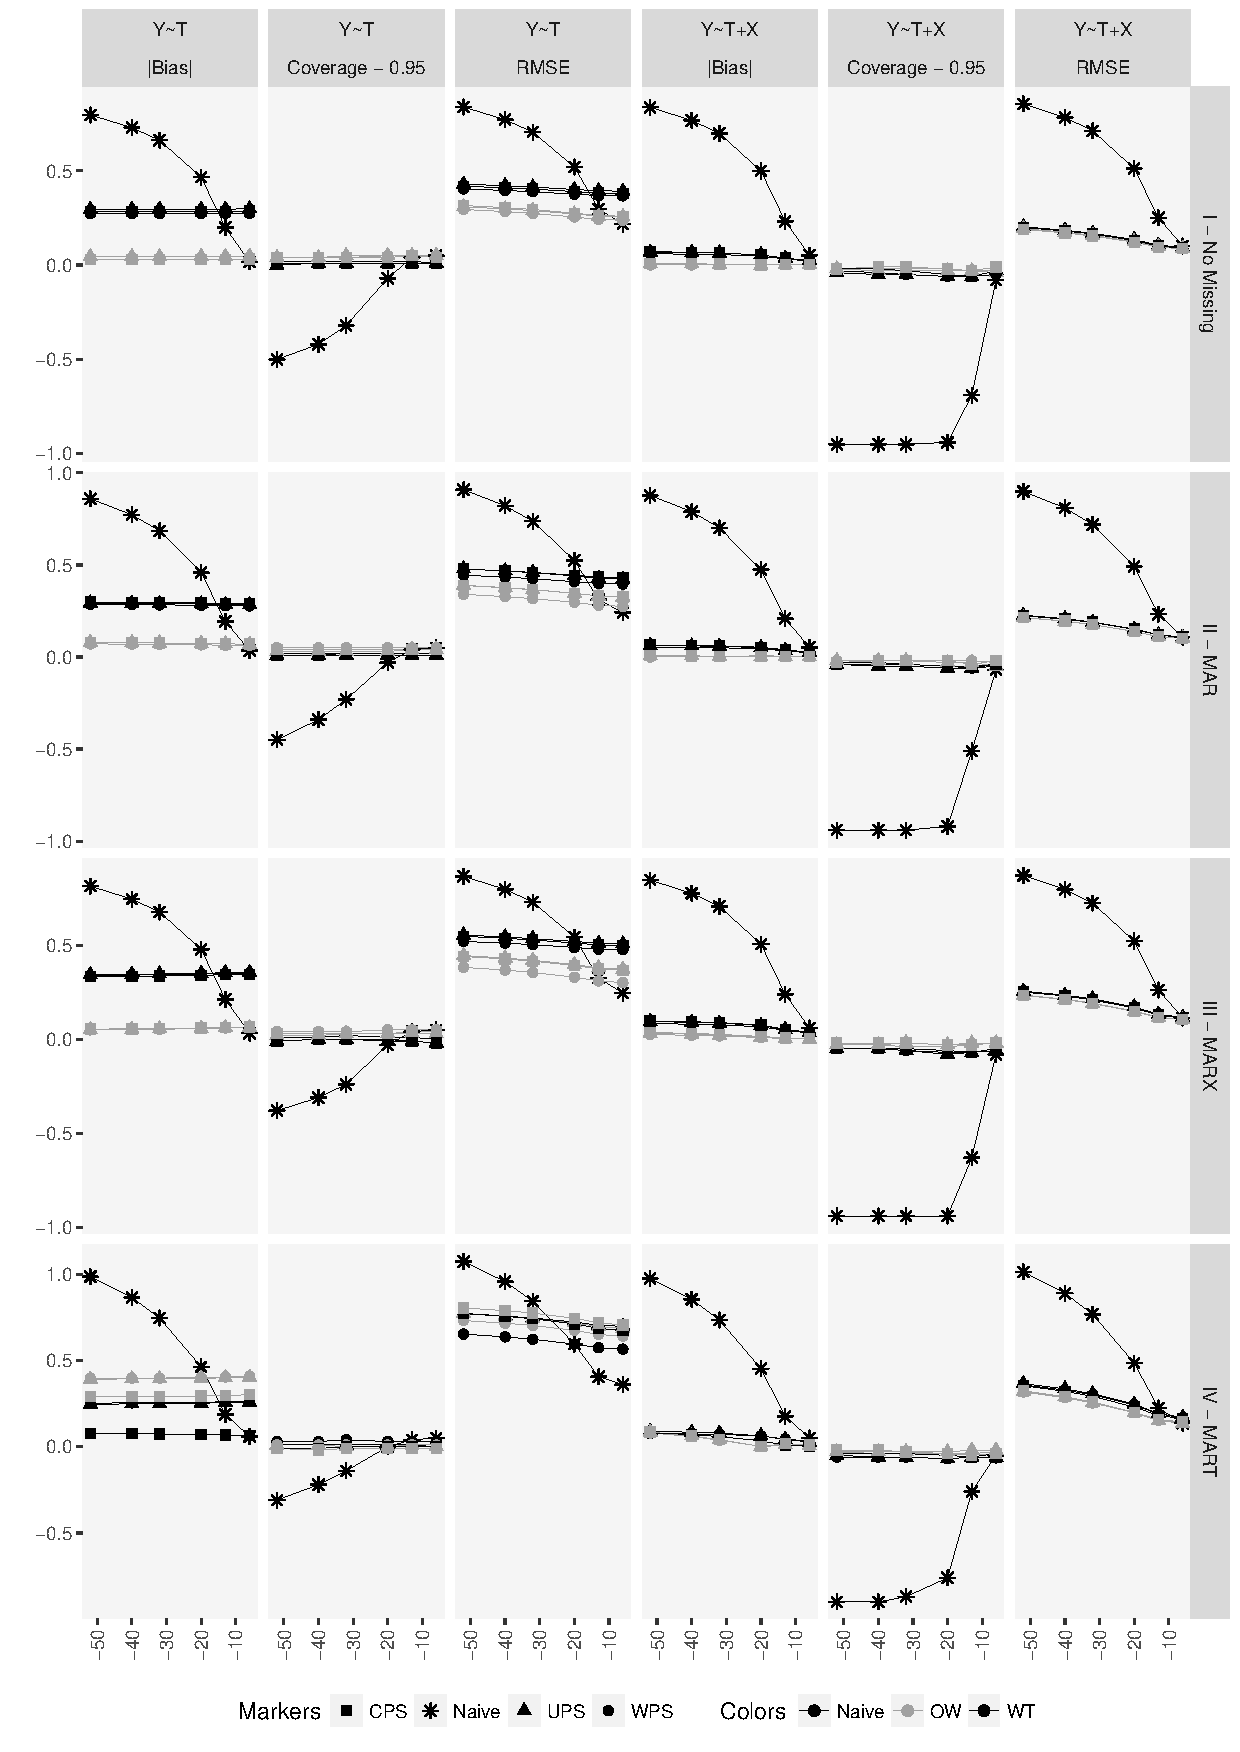
\includegraphics[scale=0.63]{Scenario3_v2.pdf}
\caption{{\small{}\textbf{Results: Scenario 3.} Bias in absolute value, coverage and root mean squared error (RMSE) as functions
of the \% difference between the SATT and PATT (simulation study).Each marker represents how the survey weights were incorporated in estimation of the propensity score model: (\mytriangle{black}) survey weights were not used in the estimation of the propensity score model, but the sample weights are used in the computation of the SMD after matching, (\mycircle{black}) survey weights were incorporated in a weighted estimation of the propensity score model and (\mysquare{black})  survey weights were used as a covariate in the estimation of the propensity score model. Black lines  show the results when the wight transfer is implemented, gray lines show the results when the original survey weights are used. Results for the Naive estimator are displayed using a black asterisk.}}
\label{Scenario3} 
\end{figure}

\bibliographystyle{biorefs}
\bibliography{refs}
\end{document}